\chapter{Approccio proposto}
\label{chap:approccio}
\vspace{1cm}
Nel capitolo \ref{chap:SOA} sono state descritte alcune soluzioni proposte 
relative al lavoro oggetto di questa tesi, in particolare algoritmi esatti ed
euristici di ottimizzazione atti a risolvere il problema di mapping e 
scheduling, congiuntamente o separatamente. Alla luce delle limitazioni dei 
lavori presentati è stato spiegato il motivo per cui si rende necessario questo 
lavoro integrato nel progetto \ac{FASTER}, presentato nel capitolo
\ref{chap:recComputingFASTER}.

%di sviluppo di un algoritmo che consenta di effettuare un'ottimizzazione
%multiobiettivo nello spazio delle soluzioni, che consideri la riconfigurazione
%parziale dinamica come concetto esplicito di design; tale fase esplorativa
%\`e 

In questo capitolo verrà descritto l'approccio utilizzato per risolvere il 
problema del mapping di task e successivo scheduling, tenendo in considerazione le comunicazioni ed
eventualmente le riconfigurazioni introdotte.

Il capitolo è organizzato secondo la seguente struttura: nella sezione 
\ref{sec:integrazioneToolchainFASTER} viene descritta l'integrazione 
dell'algoritmo di scheduling con il componente che gestisce il mapping dei task, 
con accenni alle interfacce esterne che collegano il componente 
con gli altri strumenti utilizzati nella toolchain di \acs{FASTER}; la sezione 
\ref{sec:panoramicaMetodologia} descrive ad alto livello il funzionamento 
dell'algoritmo di esplorazione delle soluzioni e dell'algoritmo di scheduling
presente al suo interno, fornendo una panoramica delle fasi in cui questi si dividono;
% TODO trovare sezioni per ACO
la sezione \ref{sec:euristicaSceltaTask} contiene una descrizione 
dettagliata della fase più delicata del procedimento di scheduling, la scelta 
del task migliore da considerare ad ogni passo di decisione; nella sezione 
\ref{sec:elementiComunicazioneGestioneMemoria} vengono introdotti i modelli di 
comunicazione supportati dall'algoritmo proposto e una possibile allocazione 
statica della memoria per i task di computazione, svolta contemporaneamente allo 
scheduling; infine, la sezione \ref{sec:osservazioniConclusive} fornisce un 
riepilogo dei concetti importanti presentati in questo capitolo.


\section{Integrazione nella toolchain di \acs{FASTER}}
\label{sec:integrazioneToolchainFASTER}

Come descritto nel precedente capitolo, l'obiettivo del progetto europeo 
\ac{FASTER} è fornire un framework per la sintesi ad alto livello di 
applicazioni, scritte in linguaggio di programmazione C, su vari dispositivi 
riconfigurabili; la toolchain che permette di realizzare questa sintesi è 
composta da varie fasi eseguite in sequenza. Ogni fase deve essere il più 
possibile self-contained, ovvero deve poter essere invocata separatamente e non 
deve avere nozioni sul funzionamento interno delle altre fasi.

Condizione necessaria perchè ciò accada è la definizione di specifiche 
interfacce per ogni strumento che deve essere invocato. Ad esempio, la fase di 
mapping ha la propria interfaccia di input e di output; lo scheduler 
(invocato dall'algoritmo di esplorazione dello spazio delle soluzioni) ha 
anch'esso una interfaccia di input e una di output, contenenti tutte 
le strutture dati necessarie per l'elaborazione e per la memorizzazione delle 
informazioni calcolate dall'algoritmo, rispettivamente. 


%A livello dell'algoritmo di esplorazione delle soluzioni, dunque, si avrà un 
%flusso di lavoro come rappresentato nella figura \ref{fig:mapperWorkflow}, in 
%cui a titolo esemplificativo sono rappresentate le interfacce di input e output
%dello scheduler.

L'algoritmo di esplorazione, che si occupa dell'invocazione del tool che gestisce lo 
scheduling, è caratterizzato dalle proprie interfacce di input e output. Dato che il componente
di scheduling \`e invocato successivamente al mapping, l'output del mapper e l'interfaccia
di input dello scheduler avranno alcuni dati.

Nella prossima sezione verranno descritte le interfacce di input dell'algoritmo di esplorazione
e della fase di scheduling.

\subsection{Interfacce di input}

L'interfaccia di input dell'algoritmo di esplorazione comprende i dati relativi al
progetto correntemente aperto in \ac{FASTER}, tra cui:
\begin{itemize}
  \item descrizione dell'architettura e degli elementi di computazione, comunicazione
    e memoria presenti;
  \item descrizione del task graph che rappresenta l'applicazione e delle implementazioni
    a disposizione per realizzare la funzionalit\`a di ogni task, ognuna con la propria stima
    di risorse richieste e tempo di esecuzione.\footnote{Per implementazioni di tipo software, il tempo di esecuzione
    stimato si pu\`o ottenere tramite profiling; nel caso di implementazioni hardware \`e possibile
    ottenere le stime di performance e requisiti tramite strumenti di sintesi ad alto
    livello come \emph{Vivado HLS} \cite{VivadoHLS}.}
\end{itemize}
Oltre a questi, l'input dell'esplorazione comprende anche i vari parametri per la configurazione
dell'algoritmo, ad esempio parametri sulle metriche da utilizzare e funzioni da utilizzare per il calcolo
del loro valore, e parametri di configurazione del numero di iterazioni e del criterio di terminazione.


\begin{figure}
 \begin{minipage}[b]{0.4\textwidth}
  \begin{center}
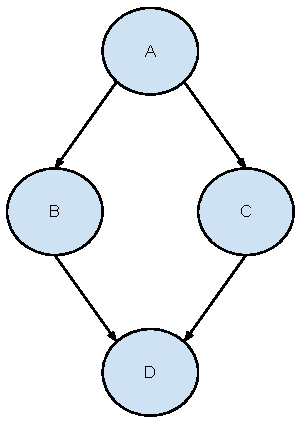
\includegraphics[width=\linewidth]{capitoli/figure/cap4/TaskGraphExample.pdf}
  \subcaption{Task graph}\label{fig:taskGraphExample2}
  \end{center}
 \end{minipage}
 \hfill
 \begin{minipage}[b]{0.5\textwidth}
  \begin{center}
   \begin{tabular}{| c | c | c |}
    \hline
    \textbf{Task} & \textbf{Componente} & \textbf{Implementazione}\\
    \hline
    A & p1 & impl\textunderscore0\\
    \hline
    B & p2 & impl\textunderscore1\\
    \hline
    C & p1 & impl\textunderscore2\\
    \hline
    D & p3 & impl\textunderscore3\\
    \hline
   \end{tabular}
   \subcaption{Lista dei mapping}\label{tab:listaMapping}
  \end{center}
 \end{minipage}
 \caption{Esempio di task graph e di lista dei mapping.}
 \label{fig:taskGraphAndMapping}
\end{figure}


L'interfaccia di input per la fase di scheduling contiene tutti i dati 
necessari all'esecuzione dello scheduler, alcuni definiti prima 
dell'invocazione del tool, altri creati o modificati durante le differenti fasi 
dell'esecuzione. In particolare, i dati definiti prima dell'invocazione sono
gli stessi dati relativi al progetto correntemente in elaborazione dalla toolchain,
e dati provenienti dall'output della fase di mapping effettuata dall'algoritmo di esplorazione.
Questi ultimi sono organizzati come una lista di triple \emph{$<$processing 
task, processing element, implementazione$>$} calcolata dal mapper, che 
specifica per ogni task:
\begin{enumerate}
 \item l'elemento di computazione che dovrà eseguire il task, può essere un 
core hardware su scheda oppure un core software (processore);\footnote{Il termine
\emph{core software} non deve essere confuso con il termine \emph{softcore} introdotto
nella sezione \ref{sec:algoritmiEuristici}, che rappresenta un core implementato su
logica riconfigurabile invece che un processore.}
 \item l'implementazione da utilizzare per l'esecuzione del task, si può 
dividere in implementazione software o hardware a seconda che il task debba 
essere eseguito su scheda o su un processore.
\end{enumerate}
Nella figura \ref{fig:taskGraphAndMapping} sono rappresentati un esempio di 
task graph e di un possibile output della fase di mapping basato su quel task graph.

Le informazioni provenienti dal mapper vengono quindi utilizzate per 
determinare se alcune aree dovranno essere riconfigurate durante l'esecuzione 
dell'applicazione oppure no, oltre a dare informazioni sull'occupazione dei 
vari componenti del dispositivo.


\subsection{Interfaccia di output}
L'interfaccia di output dell'algoritmo di esplorazione \`e costituita dalla
migliore soluzione trovata nel corso dell'esplorazione dello spazio delle soluzioni
possibili, e include l'output dello scheduler (descritto nel prossimo paragrafo),
il valore della funzione obiettivo, il numero di processing element utilizzati e
la dimensione dell'area utilizzata.

%Il compito dello scheduler è assegnare delle stime di tempo di inizio e di fine 
%esecuzione ad ogni task in modo che le precedenze imposte dal task graph
%vengano rispettate, e che nessun altro vincolo sia violato: ad esempio, 
%task che devono essere eseguiti sullo stesso componente non possono avere tempi 
%di esecuzione sovrapposti.

L'interfaccia di output dello scheduler è composta da tutte le informazioni
calcolate dall'algoritmo:
\begin{itemize}
 \item una rappresentazione in forma di \emph{diagramma di Gantt}, che delinea 
per ogni componente quando questo è occupato nell'esecuzione di un task;
 \item per ogni task, una lista delle informazioni riguardanti lo scheduling, 
ad esempio il tempo d'esecuzione stimato, il componente su cui deve essere 
eseguito, l'implementazione che ne caratterizza l'esecuzione e le stime di 
inizio e fine esecuzione che gli sono state assegnate;
 \item le informazioni relative agli indirizzi di memoria assegnati ai task
 di computazione.
\end{itemize}

Nella prossima sezione verrà spiegato in dettaglio il flusso di 
esecuzione dell'algoritmo di esplorazione (mapping e scheduling), e come le
interfacce vengono utilizzate durante l'elaborazione.


\section{Panoramica della metodologia}
\label{sec:panoramicaMetodologia}

% FIXME cambiare figura mettendo quella della formichina?
\begin{figure}[t]
  \begin{center}
    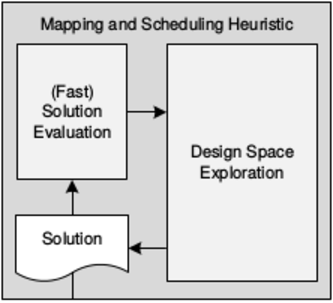
\includegraphics[width=0.5\textwidth]{./capitoli/figure/cap4/Methodology.pdf}
    \caption{Panoramica del flusso dell'algoritmo di esplorazione.}
    \label{fig:mapperWorkflow}
  \end{center}
\end{figure}

In figura \ref{fig:mapperWorkflow} \`e rappresentato ad alto livello il workflow
dell'algoritmo euristico di mapping e scheduling, costituito da un ciclo di:
\begin{enumerate}
  \item calcolo di una possibile soluzione in termini di mapping e scheduling;
  \item calcolo dei valori delle metriche relativi alla soluzione appena calcolata.
\end{enumerate}

In questa sezione viene descritto il funzionamento dell'algoritmo proposto e le 
fasi in cui esso si articola, con una spiegazione dettagliata della struttura 
di ogni fase e del flusso di lavoro completo dell'algoritmo.


%%% FIXME: color
\begin{figure}
 \begin{center}
  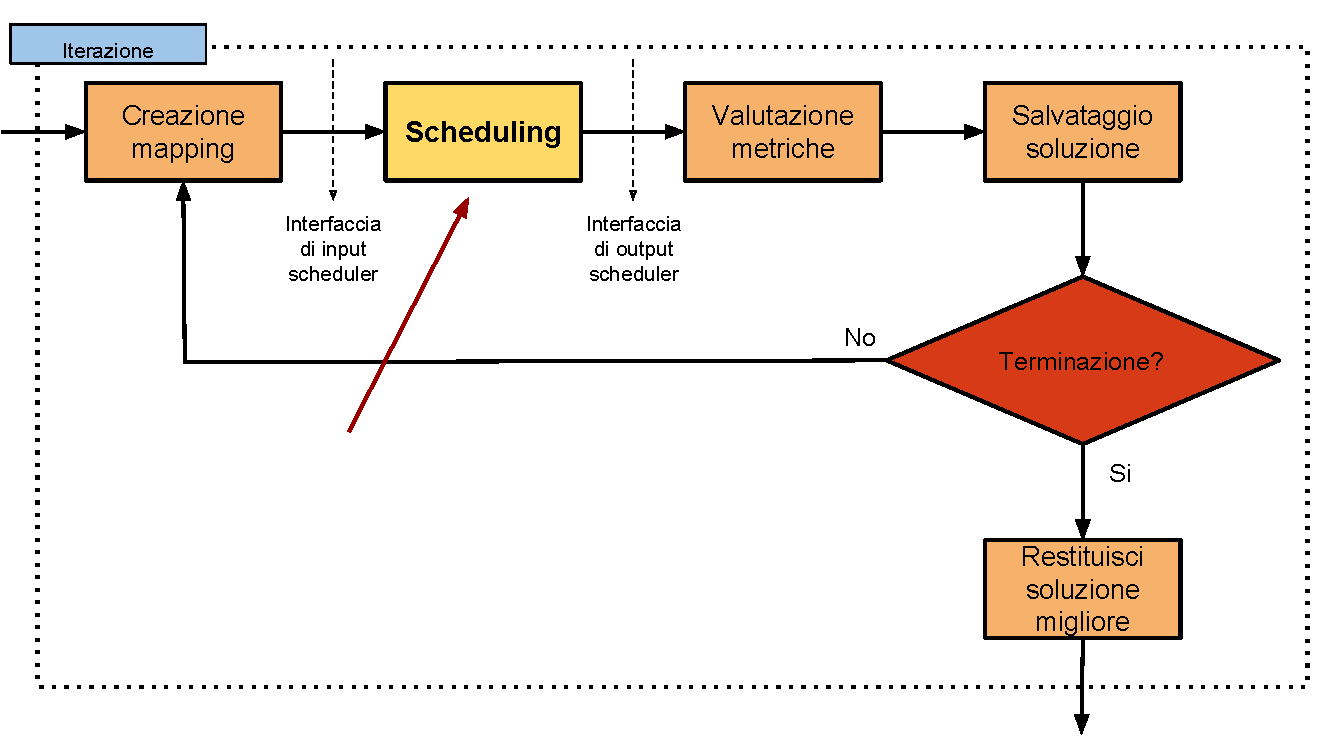
\includegraphics[width=0.9\textwidth]{capitoli/figure/cap4/MapperWorkflow.pdf}
  \caption{Fasi dell'algoritmo di esplorazione.}
  \label{fig:flussoDettagliatoACO}
 \end{center}
\end{figure}


\subsection{Algoritmo di esplorazione}
Una rappresentazione dettagliata del flusso di lavoro dell'algoritmo di
esplorazione \`e mostrata in figura \ref{fig:flussoDettagliatoACO}: \`e
possibile vedere come in seguito al calcolo di una soluzione, eseguite le fasi
di mapping e scheduling, le varie metriche vengano valutate e la soluzione
aggiunta alla lista. Una volta che il criterio di terminazione \`e soddisfatto,
l'esplorazione termina e la soluzione migliore (quella con funzione obiettivo pi\`u
bassa) viene restituita. In figura \ref{fig:flussoDettagliatoACO} sono rappresentate
anche le interfacce di input e output della fase di scheduling, descritte in precedenza.

L'esplorazione dello spazio delle soluzioni, in inglese \ac{DSE},  \`e basata su un algoritmo
meta-euristico chiamato \acf{ACO}. L'algoritmo \ac{ACO}, di recente sviluppo, è stato inizialmente 
utilizzato per risolvere il problema del commesso viaggiatore (\acs{TSP}) 
\cite{AntSystem} e poi esteso anche ad altri problemi di ottimizzazione 
combinatoria.

Nella fattispecie, l'algoritmo cerca di riprodurre il procedimento seguito da una colonia di 
formiche alla ricerca di cibo; la colonia deve poter giungere al cibo seguendo 
il percorso più breve, che rappresenta una soluzione (subottima) trovata.
Quando una colonia va alla ricerca di cibo, tutte le formiche partono dalla 
colonia seguendo direzioni casuali, lasciando una traccia di 
\emph{feromone}\footnote{Il feromone è una sostanza emessa da alcuni esseri 
viventi con funzione di segnalare qualcosa agli individui riceventi 
della stessa specie: una traccia, un pericolo, una modificazione 
comportamentale per il ricevente.} sul loro cammino. La traccia di feromone 
evapora con il tempo, ma il percorso più breve dalla colonia al cibo (la soluzione ottima) conterrà 
sempre una quantit\`a maggiore di feromone, perch\`e il tempo richiesto dalle formiche
per percorrerlo \`e minore. Questo implica che pi\`u formiche saranno attratte da
quel percorso invece che da altri, rilasciando a loro volta feromoni che
``rinforzeranno'' il percorso. In un certo senso, l'ammontare di feromoni su un cammino
indica \emph{globalmente} quanto quel cammino sia buono per raggiungere l'obiettivo.

L'euristica si basa sull'astrazione di un agente, la ``formica'', che esplora
in maniera stocastica lo spazio delle soluzioni, descritto come una sequenza di possibili scelte.
A ogni iterazione dell'algoritmo, un certo numero di agenti viene istanziato;
a ogni passo di scelta, ogni agente calcola tutte le possibili scelte e le ordina secondo un
criterio che guida l'algoritmo nella ricerca della soluzione, man mano che si procede con
le iterazioni. La regola per l'ordinamento della soluzione si basa su due euristiche:
\begin{itemize}
  \item un'euristica \emph{locale}, che assegna un punteggio a una scelta dato
    lo stato corrente dell'esplorazione;
  \item un'euristica \emph{globale}, che realizza un modello per rappresentare il concetto
    di ``feromone'', applicato al problema corrente.
\end{itemize}
L'euristica locale permette all'agente, durante la costruzione della soluzione,
di compiere una decisione informata riguardo alla scelta successiva, e integra conoscenze
sul problema.

L'euristica globale, invece, permette di aggiornare la quantit\`a di feromoni
ad ogni iterazione dell'algoritmo.
In ottica stocastica, la quantità di feromone rappresenta la probabilità, per 
ciascuna decisione, di giungere a una buona soluzione.
All'inizio dell'algoritmo, la matrice dei feromoni è inizializzata con valori uniformi 
(tutte le decisioni hanno uguale probabilità), e viene aggiornata dopo ogni
iterazione esplorativa.

L'algoritmo \ac{ACO} implementa l'esplorazione in forma iterativa, sfruttando una
serie di ``generazioni di formiche''. Una \emph{generazione} \`e composta da un
numero $N$ di formiche, ognuna di esse esplora lo spazio di design e costruisce una soluzione
utilizzando i medesimi valori della matrice dei feromoni. 
Il criterio che stabilisce l'ordinamento delle scelte possibili, ad ogni passo decisionale,
\`e rappresentato da una probabilit\`a, funzione della posizione corrente nel processo decisionale, 
della destinazione da raggiungere, dell'euristica locale calcolata ogni volta 
che la probabilità è generata e dell'euristica globale. La formula per il 
calcolo della probabilità è la seguente:
\begin{equation}
 p_{x,y} = \frac{[\tau_{x,y}]^{\alpha}\cdot[\eta_{x,y}]^{\beta}}{\sum_{l \in 
\Omega_{x}}[\tau_{x,l}]^{\alpha}\cdot[\eta_{x,l}]^{\beta}}
\end{equation}
dove $x$ è la posizione corrente nel processo decisionale, $y$ è la 
destinazione della ricerca, $\eta$ è l'euristica locale legata al problema e 
$\tau$ è l'euristica globale determinata dal feromone. $\alpha$ e $\beta$ 
rappresentano i pesi che vengono dati alle due euristiche e che influenzano il 
comportamento della formica nel processo decisionale. $\Omega_x$ è l'insieme che 
contiene tutte le scelte possibili al passo corrente $x$. Alla fine di ogni generazione,
soltanto un certo numero $K$ di formiche, con $K \leq N$, sono considerate per il rinforzo
dell'euristica globale. Il rinforzo assegnato \`e proporzionale alla qualit\`a della soluzione,
e la matrice dei feromoni viene aggiornata secondo la formula
\begin{equation}
 \tau_{x,y} = (1-\rho)\cdot \tau_{x,y} + \epsilon
\end{equation}
dove $\rho$ è il \emph{fattore di evaporazione} del feromone, mentre $\epsilon$ 
rappresenta il coefficiente correttivo di rinforzo che evita di penalizzare 
tramite l'evaporazione anche le scelte migliori.

\IncMargin{1em}
\begin{algorithm}[!htbp]
\footnotesize
\SetKwData{readySet}{readySet}\SetKwData{This}{this}
\SetKwData{pTi}{$p_{T_i}$}
\SetKwData{pT}{$p_{T}$}
\SetKwData{Pi}{$P_i$}
\SetKwData{pSet}{pSet}
\SetKwData{chosenI}{chosenI}
\SetKwData{chosenT}{chosenT}
\SetKwData{chosenP}{chosenP}
\SetKwData{pIP}{$p_{I,P}$}
\SetKwData{pIiPi}{$p_{I_i, P_i}$}
\SetKwData{mappingTrace}{mappingTrace}
\SetKwData{numGenerations}{numGenerations}
\SetKwData{antsPerGeneration}{antsPerGeneration}
\SetKwData{antA}{currentAnt}
\SetKwData{Ii}{$I_i$}
\SetKwData{chosenTask}{chosenTask}
\SetKwData{iSet}{iSet}
\SetKwData{ant}{ant}
\SetKwData{chosenTrace}{choice}
\SetKwData{antMetrics}{ant.metrics}
\SetKwData{thisGenerationSolutions}{thisGenerationSolutions}
\SetKwData{bestAnts}{bestAnts}
\SetKwData{bestAnt}{bestAnt}
\SetKwData{bestAntTrace}{bestAnt.trace}
\SetKwData{antMetrics}{ant.Metrics}
\SetKwData{antObjective}{ant.Objective}
\SetKwFunction{tasksWithoutPreds}{tasksWithoutPreds}
\SetKwFunction{resolveDependencies}{resolveDependencies}
\SetKwFunction{computeMetrics}{computeMetrics}
\SetKwFunction{computeObjective}{computeObjective}
\SetKwFunction{processorsPerImpl}{processorsPerImpl}
\SetKwFunction{implsOfTask}{implsOfTask}
\SetKwFunction{add}{add}
\SetKwFunction{rouletteSelection}{roulette}
\SetKwFunction{taskHeuristic}{taskHeuristic}
\SetKwFunction{mappingHeuristic}{mappingHeuristic}
\SetKwFunction{scheduledSet}{scheduledSet}
\SetKwFunction{updateGlobalPheromones}{updateGlobalPheromones}
\SetKwFunction{selectBest}{selectBest}
\SetKwFunction{selectBestAnt}{selectSingleBestAnt}
\SetKwInOut{Input}{input}
\SetKwInOut{Output}{output}
\Input{A task graph, a reconfigurable architecture, a set of implementations}
\Output{A mapping trace, a schedule}
\BlankLine
\ForAll{\numGenerations}{

	\ForAll{\antsPerGeneration}{

		\readySet $\leftarrow$ \tasksWithoutPreds()

		\scheduledSet $\leftarrow \emptyset$
		
		\While{\readySet $\neq \emptyset$}{
			
			\BlankLine
			
			\ForAll{$T_i \in$ \readySet}{
				\pTi $\leftarrow$ \taskHeuristic($T_i$)
			}
			\chosenT $\leftarrow$ \rouletteSelection(\pT)

			\BlankLine

			\iSet $\leftarrow$ \implsOfTask(\chosenTask)
	
			\ForAll{\Ii $\in$ \iSet}{
				\pSet $\leftarrow$ \processorsPerImpl(\Ii)
				
				\ForAll{\Pi $\in$ \pSet}{
					\pIiPi $\leftarrow$ \mappingHeuristic(\Ii, \Pi)
				}
			}
			\chosenI, \chosenP $\leftarrow$ \rouletteSelection(\pIP)
			
			\chosenTrace $\leftarrow$ $<$\chosenT, \chosenI, \chosenP$>$
			
			\mappingTrace.\add(\chosenTrace)
			
			\readySet $\leftarrow$ \resolveDependencies()
		}

		\antMetrics $\leftarrow$ \computeMetrics(\antA)
		
		\antObjective $\leftarrow$ \computeObjective(\antMetrics)
		
		\thisGenerationSolutions.\add(\ant)
	}
	\bestAnts.\add(\selectBest(\thisGenerationSolutions))
	
	\updateGlobalPheromones(\bestAnts)
}

\bestAnt = \selectBestAnt(\bestAnts)
		
\Return \bestAntTrace

\caption{Pseudo-codice dell'algoritmo di esplorazione.}
\label{alg:aco}
\end{algorithm}

L'algoritmo \ref{alg:aco} riporta lo pseudo-codice dell'algoritmo di esplorazione.
Nel prossimo paragrafo si descrivono le euristiche utilizzate nel codice per effettuare
l'esplorazione dello spazio delle soluzioni, tenendo in considerazione le riconfigurazioni.


\subsubsection{Euristica per task e mapping}
Come si pu\`o vedere nel listato \ref{alg:aco}, ogni formica di ogni generazione (righe 1-2)
costruisce una soluzione, calcolando un possibile mapping, in maniera iterativa. In particolare,
i task (riga 8)  e le possibili implementazioni e processing element su cui possono essere eseguiti
(riga 14), sono scelti tramite \emph{roulette wheel selection}. La \emph{roulette wheel
selection} \`e un modo di scegliere soluzioni potenzialmente utili da un insieme di soluzioni possibili.
Viene comunemente utilizzata come operatore all'interno degli algoritmi genetici, e opera una selezione
sulla base di una probabilit\`a. Ad esempio, dato un insieme $S$ di soluzioni e una funzione che calcola
la bont\`a -- \emph{fitness} -- di una soluzione, la probabilit\`a di selezione di una soluzione
$i \in S$ \`e calcolabile come
\begin{displaymath}
  p_i = \frac{f_i}{\sum_{j=1}^{N}f_j}
\end{displaymath}
dove $N$ \`e il numero di soluzioni della popolazione $S$.

Le probabilit\`a di selezione di un task e del relativo mapping sono calcolate alla riga 7 e alla riga
13 del listato \ref{alg:aco}, rispettivamente.

\subparagraph{Euristica per i task}
La funzione per il calcolo della probabilit\`a di scelta associata a ogni task,
\verb+taskHeuristic(+$T_i$\verb+)+, ordina i task le cui dipendenze sono gi\`a state
considerate nei passi precedenti cercando di favorire quelli caratterizzati da una bassa
\emph{mobilit\`a}.\footnote{Nel contesto di questo lavoro, ci si riferisce alla mobilit\`a di un
  task come a una misura di quanto tale task sia ``vincolato'', ovvero quanto probabilmente
si colloca sul percorso critico dell'applicazione.}
Allo stesso tempo, favorisce anche i task che eseguono pi\`u velocemente rispetto agli altri.

Il valore dell'euristica locale per un task, prima di essere tradotto in probabilit\`a di
selezione, \`e calcolato nel seguente modo:
\begin{equation}
  h_i = taskSpeed_i \cdot taskMobility_i
\end{equation}
I due fattori sono calcolati tramite le formule
\begin{align*}
  taskSpeed_i &= \frac{0.5}{avgExTime_i}\\
  taskMobility_i &= (1 - \frac{1}{m_i})
\end{align*}
dove $avgExTime_i$ \`e la media dei tempi di esecuzione di tutte le implementazioni del task
e $m_i$ \`e la mobilit\`a del task, pi\`u alta se il task \`e poco vincolato e pi\`u bassa se il task
\`e relativamente pi\`u vicino al percorso critico.

Le probabilit\`a di scelta di ciascun task sono calcolate normalizzando i valori dell'euristica
su tutti i task. I valori normalizzati sono basati sul prodotto di due fattori:
\begin{equation}
  p_i = \frac{localTerm_i \cdot globalTerm_i}{heuristicSum}
\end{equation}
dove $localTerm_i$ \`e dato dall'elevamento a potenza del valore dell'euristica locale del
task per un parametro $\alpha \in (0,1)$, che rappresenta il peso dell'euristica locale
nella probabilit\`a; in maniera analoga, $globalTerm_i$ \`e dato dalla matrice globale dei feromoni,
anch'esso elevato a un parametro $\beta \in (0,1)$. Entrambi i parametri sono specificabili
dall'utente prima dell'avvio dell'esplorazione.

\subparagraph{Euristica per i mapping}
La probabilit\`a di scelta di un determinato mapping \`e calcolata dalla funzione
\verb+mappingHeuristic(+$I_i, P_i$\verb+)+, che ordina tutte le possibili coppie
$<$\emph{implementazione, processing element}$>$ tali che l'implementazione sia relativa
al task scelto in precedenza, e il processing element sia l'elemento di computazione associato
a tale implementazione. Ad esempio, sia $T_i$ il task scelto alla riga 7; come specificato
dal designer, il task $T_i$ ha due implementazioni hardware e una software, le prime
mappabili su core statici o riconfigurabili, l'ultima su un processore general-purpose.
Quindi, per ogni implementazione e processing element su cui $T_i$ pu\`o essere eseguito,
la funzione \verb+mappingHeuristic+ restituisce il punteggio relativo a tale scelta,
basandosi sullo stato corrente del mapping.
% TODO, FIXME descrivere meglio come viene effettuata tale scelta, dopo aver
% letto il codice

Al termine della procedura iterativa di costruzione della soluzione, questa viene valutata
secondo le varie metriche e ne viene calcolata la funzione obiettivo. Le soluzioni migliori
della generazione vengono salvate e si procede con una nuova generazione di formiche.
Una volta raggiunto il limite del numero di generazioni, viene selezionata come
soluzione finale la migliore tra quelle salvate al termine di ogni generazione.

\subsection{Algoritmo di scheduling}
Come accennato nella sezione precedente, l'interfaccia di input è 
caratterizzata da dati ``statici'', presenti prima dell'invocazione dello 
scheduler e da dati ``dinamici'', che subiscono modifiche oppure vengono creati 
durante l'esecuzione del tool. L'interfaccia di output è invece costruita 
incrementalmente, aggiungendo e modificando dati man mano che la computazione 
prosegue.


\begin{figure}[ht]
 \begin{center}
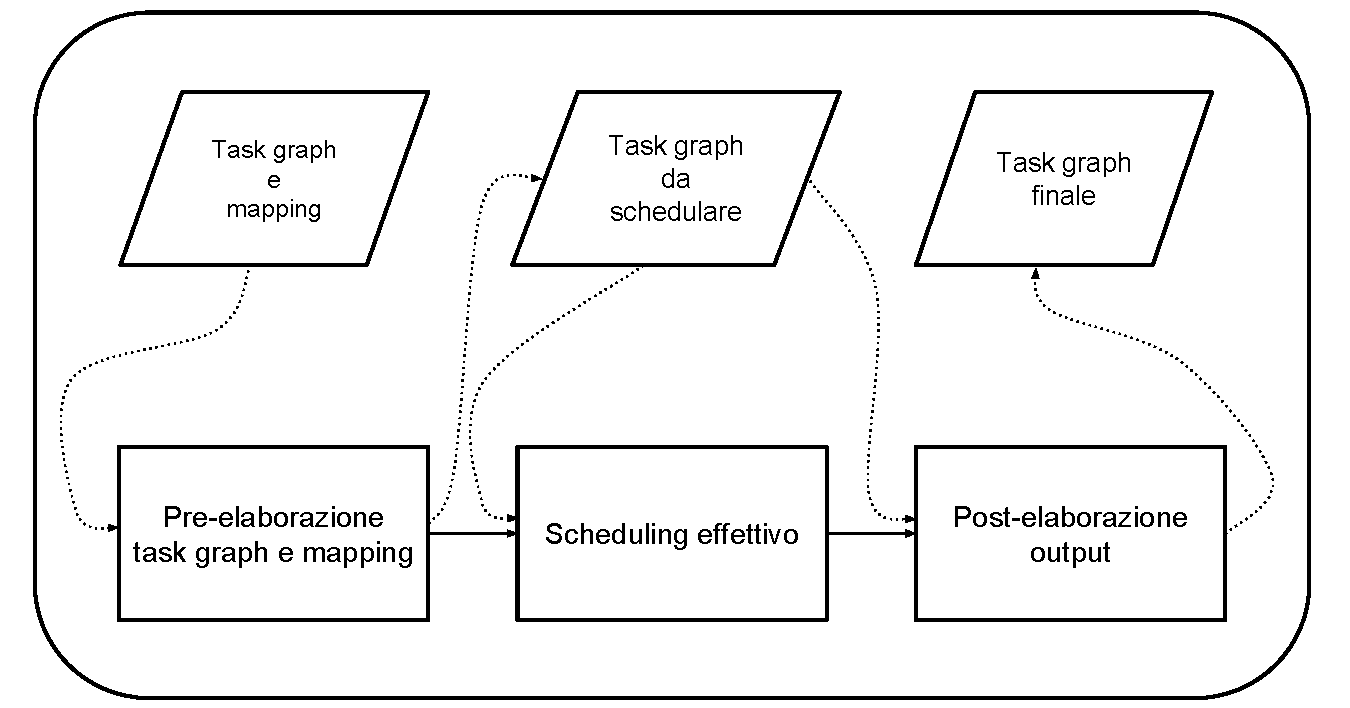
\includegraphics[width=\textwidth]
{capitoli/figure/cap4/SchedulerWorkflow.pdf}
  \caption{Flusso di lavoro dell'algoritmo di scheduling.}
  \label{fig:schedulerWorkflow}
 \end{center}
\end{figure}


La prima fase dell'algoritmo ha il compito di 
effettuare una elaborazione preliminare dei dati statici, che permetterà di 
ottenere una formulazione più specifica e dettagliata del problema; questa 
prima fase è chiamata \emph{fase di preprocessing}. La seconda fase è 
costituita dallo \emph{scheduling effettivo} dei task, utilizzando le 
informazioni calcolate in precedenza nella pre-elaborazione. La terza e ultima 
fase, pur non essendo strettamente legata all'assegnazione delle stime dei tempi 
e dell'ordine di esecuzione dei task, è fondamentale per permettere l'effettiva 
esecuzione dell'applicazione sul dispositivo riconfigurabile; consiste in una 
parziale rielaborazione dell'output prodotto dalla fase di scheduling ed è 
chiamata \emph{fase di postprocessing}.

Le tre fasi sono rappresentate nella figura \ref{fig:schedulerWorkflow}, che 
illustra il flusso di lavoro dello scheduler, con i relativi dati di input per 
ogni fase. Nelle prossime sezioni ogni fase verrà analizzata nel dettaglio.


\subsection{Fase di preprocessing}
\label{subsec:fasePreprocessing}
La fase di preprocessing è la prima ad essere eseguita dopo l'invocazione del 
tool di scheduling da parte dell'algoritmo di esplorazione; ha come obiettivo 
principale l'identificazione delle comunicazioni e delle riconfigurazioni che 
devono essere prese in considerazione per la corretta esecuzione 
dell'applicazione sul dispositivo. Un obiettivo secondario è il calcolo di 
informazioni aggiuntive che verranno poi utilizzate nella fase di scheduling 
per quanto concerne la scelta del task migliore (vedi sezione 
\ref{sec:euristicaSceltaTask}).

Per ottenere questi obiettivi, la fase di preprocessing si divide in tre 
sotto-fasi eseguite nel seguente ordine:
\begin{enumerate}
 \item aggiunta delle comunicazioni: nuovi task, detti \emph{task di 
comunicazione} vengono aggiunti al task graph originale, a rappresentare le 
comunicazioni che si verificano tra i task di computazione;
 \item aggiunta delle riconfigurazioni: può non essere richiesto e dipende 
dagli assegnamenti stabiliti dal mapper, consiste nell'introduzione di nuovi 
task, detti \emph{task di riconfigurazione}, dove necessario;
 \item calcolo delle informazioni sul percorso critico.
\end{enumerate}

\subsubsection{Aggiunta delle comunicazioni}
L'inserimento dei task di comunicazione viene fatto solamente in base 
all'analisi del task graph dell'applicazione, in quanto indipendente dal 
mapping: poichè ogni arco in tale grafo rappresenta una relazione 
produttore-consumatore tra due task,\footnote{Ovvero, denominati $i$ e $j$ i due 
task, un arco $(i,j)$ indica che l'output della computazione del task $i$ viene 
utilizzato come input per la computazione del task $j$.} ogni arco viene 
trattato come una comunicazione.

Dati due task di computazione $i$, $j$ e un 
arco $(i,j)$ nel task graph, vi sono due tipi di task di comunicazione, che si 
differenziano per come viene operato il trasferimento dei dati:
\begin{itemize}
 \item task di comunicazione di tipo \emph{WRITE}, che \emph{scrivono} 
l'output del task $i$ in una memoria;
 \item task di comunicazione di tipo \emph{READ}, che \emph{leggono} dei dati 
da una memoria e li trasferiscono come input per il task $j$. 
\end{itemize}
Stanti queste premesse, ogni arco nel task graph implica l'inserimento di 
entrambi i tipi di task di comunicazione. L'arco originale viene rimosso e 
sostituito con nuovi archi che collegano i task di computazione con i task di 
comunicazione appena inseriti, rispettando i criteri precedentemente stabiliti.


\begin{figure}
 \begin{minipage}[b]{0.4\textwidth}
  \begin{center}
   $\vcenter{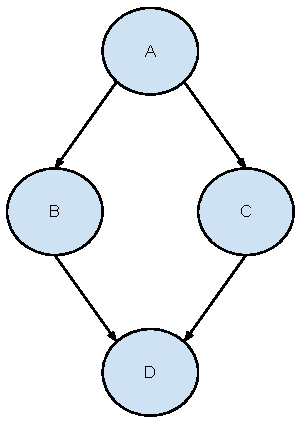
\includegraphics[width=\linewidth]
{capitoli/figure/cap4/TaskGraphExample.pdf}}$
  \end{center}
 \end{minipage}
 \hfill
 \begin{minipage}[b]{0.4\textwidth}
 \begin{center}
    $\vcenter{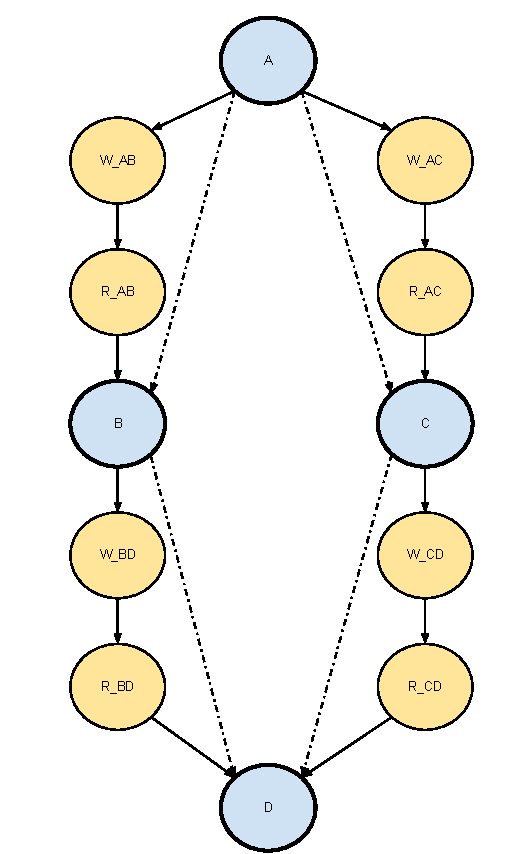
\includegraphics[width=\linewidth]
{capitoli/figure/cap4/TaskGraphCommunicationExample.pdf}}$
 \end{center}
 \end{minipage}
 \caption[Aggiunta delle comunicazioni]{Modifica del task graph in seguito all'aggiunta
 delle comunicazioni.}
 \label{fig:taskGraphCommunicationExample}
\end{figure}


Si veda la figura \ref{fig:taskGraphCommunicationExample}
per un esempio di come viene modificato il task graph della figura 
\ref{fig:taskGraphExample2} in seguito all'aggiunta dei task di 
comunicazione.\footnote{Gli archi del grafo originale sono stati 
tratteggiati per evidenziare come la struttura generale non sia cambiata ma 
siano stati soltanto introdotti nuovi nodi e archi nel grafo.}

Dopo l'inserimento dei task di comunicazione, viene eseguito l'inserimento dei 
task di riconfigurazione, qualora il particolare mapping utilizzato lo 
richieda; nel caso, si procede come descritto nel prossimo paragrafo.


\subsubsection{Aggiunta delle riconfigurazioni}
\label{sec:aggiuntaRiconfigurazioni}
L'inserimento dei task di riconfigurazione avviene in seguito all'analisi della 
lista di tuple fornita dal mapper ed è necessario nel caso in cui gli 
assegnamenti stabiliti dal mapper verifichino le seguenti condizioni:
\begin{enumerate}
 \item due task di comunicazione sono mappati sullo stesso componente 
(processing element);
 \item le implementazioni dei due task sono diverse e di tipo hardware, ovvero 
i due task devono essere eseguiti su logica riconfigurabile: questa condizione 
implica che il modulo hardware non sia riutilizzabile da parte del secondo task.
\end{enumerate}
Se queste condizioni sussistono per una qualsiasi coppia di task, allora 
un nuovo task di riconfigurazione deve essere aggiunto al grafo. Nella tabella 
\ref{tab:esempioRiconfigurazione} è illustrato un esempio di quando si 
verificano le precedenti condizioni ed è necessario introdurre un nuovo task di 
riconfigurazione.

\begin{table}[h]
\begin{center}
\begin{tabular}{| c | c | c |}
 \hline
    \textbf{Task} & \textbf{Component} & \textbf{Implementation}\\
    \hline
    A & \textcolor{red}{p1} & \textcolor{blue}{impl\textunderscore0}\\
    \hline
    B & p2 & impl\textunderscore1\\
    \hline
    C & \textcolor{red}{p1} & \textcolor{blue}{impl\textunderscore2}\\
    \hline
    D & p3 & impl\textunderscore3\\
    \hline
\end{tabular}
\caption[Mapping con riconfigurazione necessaria]{Esempio di mapping con
riconfigurazione necessaria.}
\label{tab:esempioRiconfigurazione}
\end{center}
\end{table}


L'inserimento avviene seguendo un preciso criterio per l'introduzione delle 
dipendenze: non si può semplicemente inserire il nuovo task tra i due task di 
computazione e collegarlo a questi con dei nuovi archi, è necessario tenere 
conto delle comunicazioni appena introdotte. Ad esempio, dati due task di 
computazione $i$ e $j$ anche non adiacenti, non è possibile eseguire la 
riconfigurazione prima che l'output del task $i$ sia stato salvato in memoria 
perchè i dati sarebbero sovrascritti e non più disponibili; allo stesso tempo 
e per il medesimo motivo, non è possibile eseguirla dopo che i dati siano stati 
trasferiti come input per il task $j$. Questi vincoli determinano i seguenti
criteri di assegnazione delle precedenze:
\begin{itemize}
 \item nuovi archi sono introdotti da tutti i task di comunicazione di tipo 
\emph{WRITE} uscenti dal task $i$ al task di riconfigurazione;
 \item nuovi archi sono introdotti dal task di riconfigurazione a tutti i task 
di comunicazione di tipo \emph{READ} entranti nel task $j$.
\end{itemize}


\begin{figure}
 \begin{minipage}[b]{0.4\textwidth}
$\vcenter{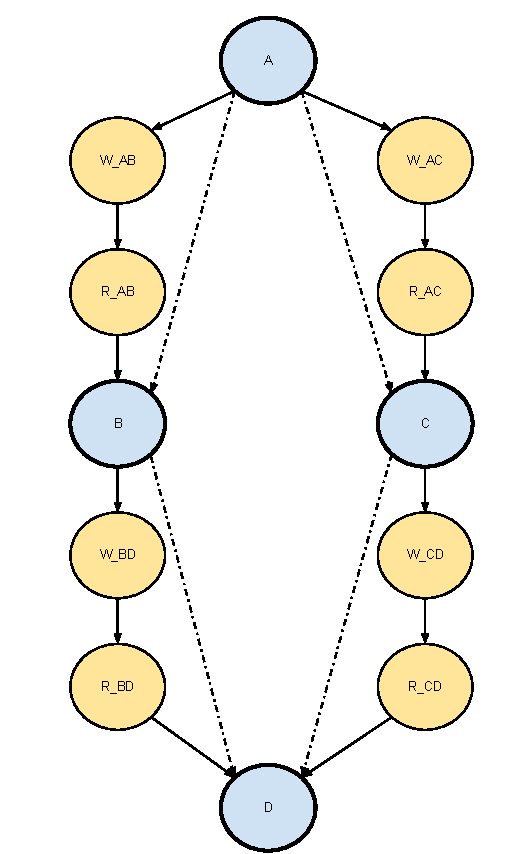
\includegraphics[width=\linewidth]
{capitoli/figure/cap4/TaskGraphCommunicationExample.pdf}}$
 \end{minipage}
 \hfill
 \begin{minipage}[b]{0.4\textwidth}
$\vcenter{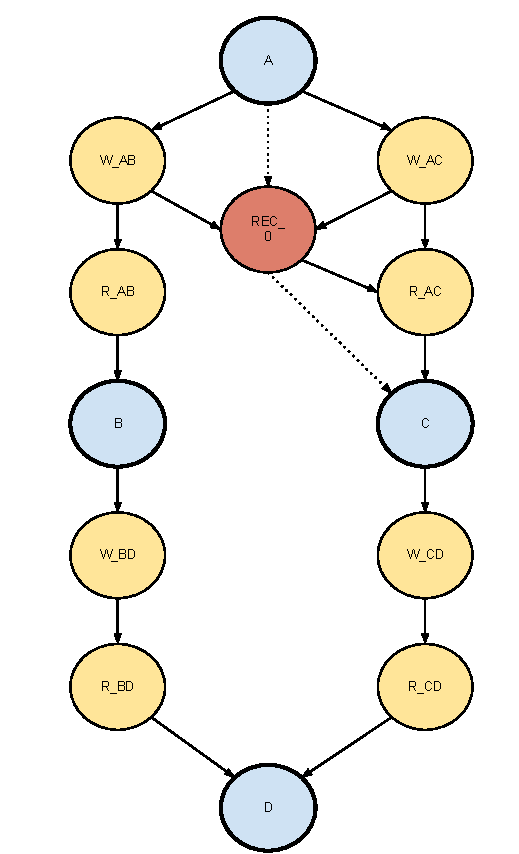
\includegraphics[width=\linewidth]
{capitoli/figure/cap4/TaskGraphCommRecExample.pdf}}$
 \end{minipage}
 \caption[Aggiunta delle riconfigurazioni]{Modifica del task graph in seguito
 all'aggiunta delle riconfigurazioni.}
 \label{fig:taskGraphCommRecExample}
\end{figure}


Nella figura \ref{fig:taskGraphCommRecExample} è rappresentata l'evoluzione del 
task graph successiva all'introduzione dei task di riconfigurazione, sulla 
base dei mapping riportati nella figura \ref{tab:listaMapping} e nella
tabella \ref{tab:esempioRiconfigurazione}. Si può vedere il nuovo task di 
riconfigurazione introdotto, di colore rosso; gli archi entranti e uscenti dal 
nuovo task impongono le precedenze sopra elencate.

Una considerazione 
aggiuntiva riguarda gli archi tratteggiati che, nel grafo sulla destra, 
collegano i due task di computazione con il task di riconfigurazione: questi 
archi vengono inseriti in ogni caso durante il preprocessing, per esplicitare 
che deve verificarsi una riconfigurazione tra l'esecuzione del task $A$ e 
l'esecuzione del task $C$. La loro introduzione non influenza tuttavia il 
funzionamento dello scheduler. Le precedenze aggiuntive introdotte dal cammino 
$A \rightarrow REC\_0 \rightarrow C$ sono infatti dominate dai cammini già 
esistenti $A \rightarrow W\_AC \rightarrow REC\_0 \rightarrow R\_AC \rightarrow 
C$ e $A \rightarrow W\_AB \rightarrow REC\_0 \rightarrow R\_AC \rightarrow C$, 
quindi la presenza di tali archi non introduce nessun ritardo e non comporta 
svantaggi rispetto alla loro assenza.

Dopo l'aggiunta dei task di riconfigurazione, l'ultimo passo della fase di 
preprocessing consiste nel calcolo delle informazioni sul percorso critico del 
task graph.


\subsubsection{Calcolo delle informazioni sul percorso critico}
Le informazioni calcolate durante questa fase vengono utilizzate per stabilire 
quali task sono sul percorso critico;\footnote{In inglese \emph{critical path}, 
avendo un grafo che simboleggia un progetto composto da attività (nodi) con 
precedenze (archi), rappresenta un cammino dal nodo iniziale al nodo finale del 
grafo costituito da attività che non possono essere ritardate senza allungare 
il tempo di esecuzione del progetto.} nella fase di scheduling vero e proprio
saranno poi utilizzate per l'assegnazione della priorità ai task.

Tali informazioni consistono in tre dati, calcolati per ogni task del grafo 
preprocessato:
\begin{itemize}
 \item istante al più presto \emph{(asap)},
 \item istante al più tardi \emph{(alap)},
 \item scarto \emph{(slack)}: differenza tra istante al più tardi e istante al 
più presto.
\end{itemize}
I task con scarto pari a $0$ fanno parte del percorso critico.

Il calcolo delle tre informazioni sopra elencate viene effettuato tramite un 
semplice algoritmo comunemente utilizzato in ricerca operativa: il \emph{metodo
del percorso critico}, in inglese \ac{CPM}.
Vengono quindi aggiunti due \emph{nodi dummy}: sorgente, collegato ai nodi del 
grafo senza predecessori e destinazione, collegato ai nodi senza successori.
Il grafo viene poi ordinato topologicamente,\footnote{Si noti che il task graph 
è aciclico quindi l'ordinamento topologico è sempre possibile.} e l'algoritmo 
\ac{CPM} viene eseguito. Lo pseudocodice dell'algoritmo di ordinamento 
topologico è illustrato nell'algoritmo \ref{alg:CPM}, dove $\delta^-(i)$ e 
$\delta^+(i)$ rappresentano il taglio entrante e il taglio uscente del nodo 
$i$, rispettivamente.

\IncMargin{1em}
\begin{algorithm}[!htbp]
 \SetKwInOut{Input}{input}\SetKwInOut{Output}{output}
 \SetKwArray{Asap}{asap}\SetKwArray{Alap}{alap}
 \SetKw{KwDownTo}{downto}
 
 \Input{Un grafo $G=(N,A)$, con $n = \vert N \vert$ e $d_i,\; \forall i = 
1,\dots,n$ durata del task $i$}
 \Output{$asap[i]$ e $alap[i],\; \forall i = 1,\dots, n$}
 \BlankLine
 \Asap{1} $\leftarrow 0$\;
 \For{$i = 2$ \KwTo $n$}{
 \Asap{i} $\leftarrow max\{$\Asap{p}$+ d_p\;:\;(p,i) \in \delta^-(i)\}$\;
 }
 \Alap{n} $\leftarrow$ \Asap{n}\;
 \For{$i=n-1$ \KwDownTo $1$}{
 \Alap{i} $\leftarrow min\{$\Alap{t}$- d_i\;:\;(i,t) \in \delta^+(i)\}$\;
 }
 \caption{Algoritmo CPM}
\label{alg:CPM}
\end{algorithm}
\DecMargin{1em}

Il calcolo delle informazioni sul percorso critico conclude la fase di 
preprocessing. Al termine di questa fase, il task graph presente 
nell'interfaccia di input dello scheduler viene sostituito con il grafo 
arricchito di comunicazioni e riconfigurazioni; le informazioni sul percorso 
critico appena calcolate sono aggiunte all'interfaccia, per essere utilizzate 
nella fase successiva.


\subsection{Fase di scheduling}
\label{subsec:faseScheduling}
La fase di scheduling effettivo gestisce l'assegnazione di tempi di inizio e 
fine dell'esecuzione di ogni task, sia esso di computazione, comunicazione o 
riconfigurazione. In particolare, la fase di scheduling assegna un ordine di 
esecuzione dei task che rispetti tutte le precedenze imposte dal task graph e 
che cerchi di minimizzare il tempo di esecuzione \emph{stimato}, a condizione
che le stime sulla durata dei task siano il più precise possibile.

\IncMargin{1em}
\begin{algorithm}[!htbp]
 \SetKwInOut{Input}{input}\SetKwInOut{Output}{output}
 \SetKwData{UnscheduledSet}{unscheduledSet}
 \SetKwData{SchedulerOutput}{schedulerOutput }
 \SetKwData{SchedulerInput}{schedulerInput}
 \SetKwData{BestTask}{bestTask}
 \SetKwData{ReadyTaskSet}{readyTaskSet}
 \SetKwData{TimeInfo}{timeInfo}
 
 \Input{the input interface of the scheduler}
 \Output{the output interface of the scheduler}
 \BlankLine
 \SchedulerOutput $\leftarrow \emptyset$\;
 \UnscheduledSet $\leftarrow$ \SchedulerInput.getTaskSet()\;
 \While{\UnscheduledSet is not empty}{
 \ReadyTaskSet $\leftarrow$ tasks with precedences satisfied\;
 \BestTask $\leftarrow$ best task to be scheduled among the ready tasks\;
 \TimeInfo $\leftarrow$ compute start/end time estimations for the best task\;
 \SchedulerOutput $\leftarrow$ \SchedulerOutput $\cup$ \TimeInfo\;
 \ReadyTaskSet $\leftarrow$ \ReadyTaskSet $\setminus$ \BestTask\;
 \UnscheduledSet $\leftarrow$ \UnscheduledSet $\setminus$ \BestTask\;
 }
 \Return{\SchedulerOutput}
\caption{Algoritmo per la fase di scheduling}
\label{alg:faseScheduling}
\end{algorithm}
\DecMargin{1em}

Come si può vedere nell'algoritmo \ref{alg:faseScheduling}, la fase di 
scheduling è costituita principalmente da un ciclo ripetuto finchè vi sono 
task che non sono ancora stati schedulati (riga 3). A ogni ripetizione del ciclo viene 
prima aggiornato l'insieme dei task che sono ``pronti'' per l'assegnazione dei 
tempi (riga 4), ossia i task le cui precedenze sono state tutte già considerate. Tra 
questi, tramite un'opportuna euristica di scelta (vedi sezione 
\ref{sec:euristicaSceltaTask}) viene eletto il miglior task da considerare al 
passo corrente (riga 5); a questo vengono poi assegnate le stime dei tempi, 
successivamente inserite nell'interfaccia di output dello scheduler e nel 
diagramma di Gantt dei componenti occupati (riga 6-7).

I dati di output dello scheduler vengono poi restituiti all'algoritmo di 
esplorazione che ha invocato il tool, e possono essere usati per avere una 
stima del tempo totale di esecuzione dell'applicazione.


\subsection{Fase di postprocessing}
Il postprocessing consiste in una rielaborazione dei dati di output dello 
scheduler, effettuata separatamente in quanto i dati prodotti in output da 
questa fase devono essere utilizzati solamente dal runtime manager per gestire 
l'esecuzione dell'applicazione.

\paragraph{Ruolo del runtime manager}
Poichè lo scheduler assegna degli istanti di inizio e fine dei task basati 
puramente su delle \emph{stime}, non vi è alcuna garanzia che tali istanti 
vengano rispettati nel corso di una reale esecuzione dell'applicazione sulla 
piattaforma riconfigurabile. Ciò vale soprattutto per i task la cui
durata di esecuzione è fortemente dipendente dalla quantità di dati da 
scambiare, da possibili conflitti sul BUS o sul canale di comunicazione 
utilizzato che rendono necessario serializzare le esecuzioni nel caso di 
task di comunicazione, oppure dalla dimensione dell'area da configurare e 
dalle caratteristiche dell'architettura sottostante nel caso di task di 
riconfigurazione.

Di fronte a questi errori nelle stime, non si può ritenere accurato il piano di 
esecuzione formulato dallo scheduler sotto forma di diagramma di Gantt; è 
necessario dunque che un componente si faccia carico dell'esecuzione dei vari 
task, lanciandone di nuovi quando i predecessori sono terminati: tale 
componente è il \emph{runtime manager}. Il ruolo del runtime manager è quello 
di coordinare le esecuzioni di tutti i task, rispettando le precedenze imposte 
dal grafo e l'ordine stabilito dallo scheduler. Il runtime manager \`e un componente
a parte che gestisce l'esecuzione dell'applicazione, ordinando i task come stabilito
dallo scheduler. Per fare ci\`o, nella fase di postprocessing lo scheduler esplicita
l'ordine di scheduling.

\begin{figure}
 \begin{minipage}[b]{0.45\textwidth}
  $\vcenter{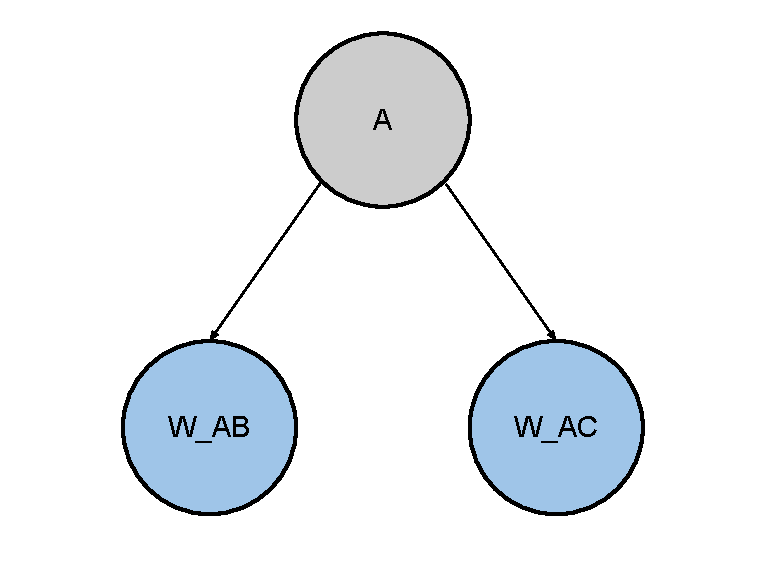
\includegraphics[width=\linewidth]
  {capitoli/figure/cap4/SchedulingConflict.pdf}}$
  \subcaption{Prima della risoluzione}
  \label{fig:schedulingConflictA}
 \end{minipage}
 \hfill
 \begin{minipage}[b]{0.45\textwidth}
  $\vcenter{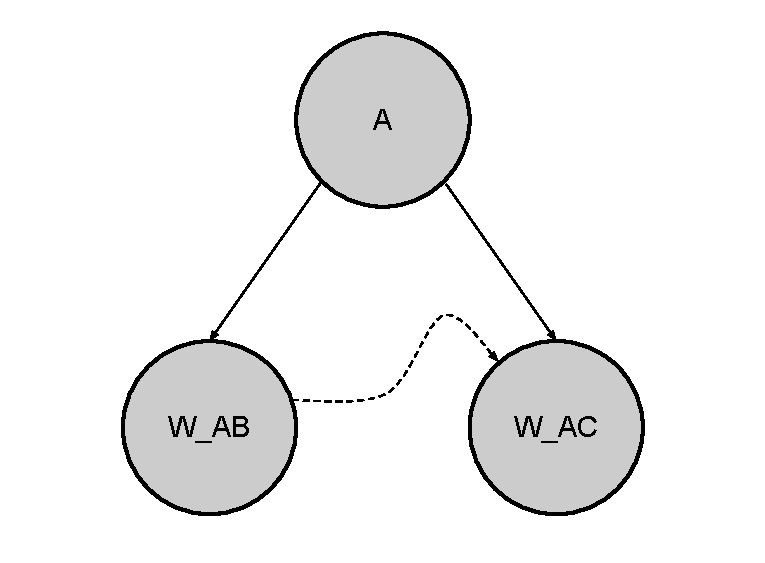
\includegraphics[width=\linewidth]
  {capitoli/figure/cap4/SchedulingConflictResolved.pdf}}$
  \subcaption{Dopo la risoluzione}
  \label{fig:schedulingConflictB}
 \end{minipage}
 \caption[Risoluzione di un conflitto tra due task]{Esempio di risoluzione di un
 conflitto tra due task.}
\label{fig:schedulingConflict}
\end{figure}

\paragraph{Definizione dell'ordine di scheduling}
Durante l'esecuzione dell'algoritmo di scheduling illustrato nella sezione 
\ref{subsec:faseScheduling} si possono avere più task eleggibili per essere 
schedulati nello stesso passo, ovvero più task con le stesse precedenze 
soddisfatte. Si consideri la figura \ref{fig:schedulingConflict} per un 
semplice esempio di conflitto tra due task. La figura 
\ref{fig:schedulingConflictA} rappresenta una parte del task graph, 
nell'ipotesi che al passo corrente il task $A$, di colore grigio, sia già stato 
schedulato mentre i due task di comunicazione $W\_AB$ e $W\_AC$, di colore 
azzurro, siano eleggibili per il passo di scheduling successivo. Quando questa
situazione si verifica, l'algoritmo deve effettuare una decisione su quale 
task sia meglio considerare per primo; tale scelta esplicita una relazione 
d'ordine tra i task in conflitto, rappresentata da un arco aggiuntivo inserito 
nella fase di postprocessing. La figura \ref{fig:schedulingConflictB} 
rappresenta l'arco aggiuntivo inserito tra i due task di comunicazione, 
nell'ipotesi che nella fase di scheduling il task $W\_AB$ sia stato scelto
prima di $W\_AC$.

È importante evidenziare come i conflitti effettivi si abbiano solo tra task 
che sono eleggibili per lo scheduling in uno stesso passo. Inoltre, è sempre possibile 
che più task eleggibili durante lo stesso passo vengano poi eseguiti in 
parallelo, a prescindere dall'ordine con cui sono stati considerati 
dall'algoritmo; si ha un vero conflitto solo quando la loro esecuzione implica 
l'utilizzo di uno stesso componente. In tal caso, infatti, le esecuzioni devono 
necessariamente essere serializzate.

\paragraph{Analisi dell'output dello scheduler}
I conflitti descritti nel precedente paragrafo sono ricavati durante la fase di
postprocessing dall'analisi del comportamento tenuto dallo scheduler.
La lista (ordinata) dei task selezionati per lo scheduling viene analizzata; nel
corso dell'analisi vengono tracciati nuovi archi seguendo l'ordine dei task nella
lista. In questo modo le informazioni sull'ordine scelto dallo scheduler vengono
incluse nel task graph finale, sotto forma di precedenze aggiuntive.

\paragraph{Scrittura dei dati su file XML}
Dopo aver analizzato il diagramma di Gantt e aver aggiunto gli archi seguendo 
l'ordine di scheduling, le informazioni rilevanti per il runtime manager 
vengono scritte nel file XML del progetto di \ac{FASTER}. I dati scritti sono:
\begin{itemize}
 \item tutte le implementazioni usate dai task che compongono il task graph 
finale, incluse eventuali implementazioni aggiuntive create ex novo per i task di 
comunicazione e di riconfigurazione;
 \item la lista dei mapping fornita dal mapper per i task di computazione, con 
mapping aggiuntivi per i task di comunicazione e riconfigurazione, che 
specificano l'implementazione da utilizzare e il componente su cui verranno 
eseguiti (componenti di comunicazione per i primi, controllore della 
riconfigurazione per i secondi);
 \item informazioni sul task graph finale, cioè con ordine di scheduling 
esplicito.
\end{itemize}

Tutte queste informazioni verranno poi utilizzate dal runtime manager per 
gestire l'effettiva esecuzione dell'applicazione.

Nella prossima sezione verrà descritta la parte più importante dell'algoritmo 
di scheduling, ossia la scelta di quale task è meglio considerare ad ogni 
passo.


\section{Euristica di scelta dei task}
\label{sec:euristicaSceltaTask}
In questa sezione viene spiegato come l'algoritmo di scheduling opera ad ogni 
passo la scelta di quale task è più conveniente considerare per l'assegnazione 
dei tempi, così da minimizzare la lunghezza totale dello schedule finale.

\paragraph{Utilizzo di un algoritmo euristico}
Come visto nel capitolo \ref{chap:SOA}, è stato preferito l'utilizzo di un 
algoritmo euristico basato su una lista con uno scheduling effettuato 
iterativamente e in maniera incrementale, rispetto a una euristica 
esplorativa/evolvibile, che richiede un tempo di esecuzione superiore prima di 
giungere a risultati accettabili e rischia di generare molte soluzioni non 
applicabili. Allo stesso tempo, il procedimento di scegliere un task ad ogni 
passo sulla base di una determinata priorità, pur essendo molto veloce 
rappresenta una scelta \emph{greedy}, che in generale non garantisce il 
raggiungimento di obiettivi accettabili.

Per questo è importante considerare diversi fattori e combinarli; sulla 
base di conoscenze pregresse è possibile identificare comportamenti 
ricorrenti che si verificano durante l'esecuzione di una generica applicazione, 
ad esempio possibili colli di bottiglia nell'esecuzione. Queste regolarità 
riscontrabili portano alla formulazione di diversi parametri che possono essere 
combinati nel calcolo della priorità che caratterizza ogni task, creando una 
funzione di priorità ``pesata'' rispetto alle possibili cifre di merito. Questo 
è l'approccio alla base dell'euristica utilizzata per la scelta dei task che 
viene illustrata in questa sezione.

\paragraph{Garanzia di applicabilità delle soluzioni generate}
L'algoritmo di scheduling proposto permette di evitare che vengano generate 
delle soluzioni \emph{infeasible}, soluzioni che violino i vincoli sul tempo di 
esecuzione (per esempio nel caso di tempi di esecuzione sovrapposti per task 
mappati sullo stesso componente), oppure che siano caratterizzate da un mancato 
rispetto delle precedenze tra i task del grafo.

Si assiste quindi alla generazione di una soluzione sempre valida per 
costruzione, poichè i task presi in esame ad ogni passo dall'euristica di 
scelta sono soltanto quelli le cui precedenze siano già state considerate. 
Questa caratteristica dell'algoritmo, combinata a una veloce euristica di scelta 
dei task, permette di ottenere in un tempo molto breve una soluzione che non 
viola nessun vincolo e che fornisce una stima del tempo di esecuzione fedele, 
nell'ipotesi che le stime dei tempi di esecuzione siano ragionevolmente 
affidabili.


\subsection{Funzionamento}
L'algoritmo per la scelta del task migliore viene invocato a ogni passo di 
scheduling, e opera su una lista aggiornata di task le cui precedenze sono 
soddisfatte.

Appena inizia l'esecuzione dell'algoritmo viene effettuata un'analisi 
preliminare della lista dei task per determinare se la lista contiene un solo 
elemento, ad esempio nel caso in cui si stia esaminando il primo nodo del 
grafo. Se si verifica questa situazione, allora l'unico elemento della lista è 
selezionato come task migliore. Nel caso in cui la lista contenga più di un 
elemento, è necessario procedere al calcolo delle priorità.

Viene eseguito un ciclo su tutta la lunghezza della lista, ad ogni passo del 
ciclo si calcola la priorità del task secondo il procedimento descritto nella 
prossima sezione; la priorità viene confrontata con la massima priorità trovata 
fino a quel momento. Dopo che tutti i task sono stati presi in esame, il task 
con la massima priorità in assoluto viene selezionato per l'assegnazione dei 
tempi, e l'algoritmo termina.

% TODO scrivere del caching delle priorità

\subsection{Calcolo delle priorità}
Il calcolo della priorità di un task dipende dal suo tipo; diverse regole e 
modi per assegnare la priorità sono utilizzati a seconda che il task sia di 
computazione, comunicazione o riconfigurazione. Anche l'implementazione 
utilizzata per i task di computazione riveste un ruolo importante per definire 
come calcolarne la priorità.

\subsubsection{Task con implementazione software}
I task con implementazione di tipo software non possono essere eseguiti su 
scheda, bensì vengono mappati su un processore general-purpose. Partendo da 
questo presupposto, la metrica utilizzata per calcolare la priorità di un task 
mappato con implementazione software è basata sulle informazioni sul percorso 
critico. In questo ambito diventano rilevanti tali informazioni, calcolate 
in precedenza durante la fase di preprocessing.

A seconda che il task sia o meno sul percorso critico del grafo, e in 
base all'eventuale scarto se così non è, viene calcolata la priorità del task 
di computazione. La funzione di calcolo della priorità dei task di computazione 
con implementazione software diventa quindi
\begin{equation} \label{eq:softwarePriority}
 f=C*CPInfo
\end{equation}
dove $C$ rappresenta un parametro costante e $CPInfo$ le informazioni sul 
percorso critico.

\subsubsection{Task con implementazione hardware}
Nel caso di task che devono essere eseguiti su logica riconfigurabile, quindi 
mappati su implementazioni di tipo hardware, vengono utilizzate tre metriche:
\begin{enumerate}
 \item informazioni sul percorso critico, come nel caso dei task con 
implementazione di tipo software;
 \item l'istante di inizio al più presto, o \emph{\ac{EST}}: rappresenta 
l'istante al più presto nel quale il task può iniziare l'esecuzione;
 \item l'istante di fine al più presto, o \emph{\ac{EFT}}.
\end{enumerate}
La funzione di calcolo della priorità risulta quindi diversa rispetto alla 
\ref{eq:softwarePriority}, assumendo la forma
\begin{equation} \label{eq:hardwarePriority}
 f=-A*EST - B*EFT + C*CPInfo
\end{equation}
dove $A$, $B$ e $C$ sono parametri fissati e $CPInfo$, $EST$ e $EFT$ sono le 
tre metriche sopra elencate.

Nei prossimi paragrafi viene descritto come si calcolano le tre metriche 
utilizzate nelle funzioni \ref{eq:softwarePriority} e \ref{eq:hardwarePriority}.

\paragraph{Informazioni sul percorso critico}
Il calcolo della metrica relativa al percorso critico si basa sulle 
informazioni riguardanti lo \emph{scarto} (slack) del task. I dati sugli 
scarti di tutti i task sono stati calcolati durante la fase di preprocessing, 
e sono disponibili in quanto inseriti nell'interfaccia di input dello scheduler.

Si fissa una soglia per lo scarto al di sotto della quale si considera il task 
come facente parte del percorso critico; al task si assegna quindi la massima 
priorità per questa cifra di merito se il suo scarto è sotto soglia. La 
definizione di una soglia permette all'algoritmo di essere meno rigido nel 
controllo dello scarto di un task, che viene così considerato come critico anche 
se il suo scarto è di poco superiore a $0$, invece che considerare critici 
solamente task con scarto esattamente pari a $0$.

Se, invece, lo scarto del task supera la soglia, si considera il logaritmo di 
tale scarto. Il valore della cifra di merito è così calcolato:
\begin{equation}
 CPInfo = \begin{cases}
           MAX & \mbox{se } 0 \leq s \leq THRESHOLD\\
           \frac{1}{log_2\left(s\right)} & \mbox{se } s > THRESHOLD
          \end{cases}
\end{equation}
dove $s$ è lo scarto del task.

\paragraph{Earliest Start Time}
L'istante al più presto nel quale il task può iniziare l'esecuzione, senza 
contare possibili conflitti nell'utilizzo dei componenti, è concettualmente 
uguale al tempo \emph{asap}, anch'esso calcolato nella fase di preprocessing 
come lo scarto. Il valore della cifra di merito è così calcolato:
\begin{equation}
 EST = \begin{cases}
        0 & \mbox{se } asap = 0\\
        log_2\left(asap\right) & \mbox{se } asap > 0
       \end{cases}
\end{equation}
Si è deciso di utilizzare il logaritmo in modo da non penalizzare 
significativamente task che hanno un EST più elevato rispetto a task con un EST 
minore. Il logaritmo infatti permette di basarsi sulla differenza tra gli ordini 
di grandezza in base $2$.
% TODO spiegare cosa l'est permette di considerare

\paragraph{Earliest Finish Time}
L'istante al più presto in cui il task termina l'esecuzione è calcolato come la 
stima asap del task, a cui viene sommato il tempo di esecuzione stimato.

Il valore di questa metrica è così calcolato:
\begin{equation}
 EFT = log_2\left(asap + eTime\right)
\end{equation}
Si noti che il caso in cui l'argomento del logaritmo abbia valore $0$ non è 
gestito, poichè il tempo di esecuzione di un task di computazione è supposto 
non nullo, e l'unico caso in cui si abbia una stima $asap$ pari a $0$ si 
verifica nell'analisi dei task iniziali, che si suppone siano sempre task di 
computazione.

Valgono considerazioni analoghe rispetto alla precedente cifra di merito 
per quanto concerne l'uso del logaritmo nel calcolo del valore.
% TODO spiegare cosa l'eft permette di considerare

\subsection{Regole aggiuntive}
Oltre al calcolo delle varie metriche presentato nella precedente sezione, sono 
state introdotte delle regole aggiuntive che modificano i valori delle cifre di 
merito e, di conseguenza, della priorità finale dei task. Queste regole non 
operano avendo conoscenza isolata a livello del singolo task, bensì agiscono in 
base al comportamento tenuto in precedenza dall'algoritmo o considerando anche 
altri task. L'aggiunta di queste regole consente quindi all'algoritmo di 
effettuare scelte più ``intelligenti'' nella scelta dei task migliori da 
schedulare.

\subsubsection{Fattore di degrado}
La prima di queste tecniche è l'introduzione di un \emph{fattore di degrado} 
(in inglese \emph{decay factor}). Può capitare che, nel corso dell'esecuzione 
dello scheduler, venga data sempre massima priorità ai task sul percorso 
critico, che vengono quindi scelti dall'euristica come migliori a ogni passo di 
scheduling. Laddove vi siano molti conflitti di mapping tra i task critici
e altri task, schedulare i task sul percorso critico per primi
può portare al verificarsi di un collo di bottiglia nell'utilizzo delle 
risorse, che vengono occupate prevalentemente da task che si trovano sul 
percorso critico, mentre altri task non possono essere eseguiti per la continua 
occupazione delle risorse su cui questi sono mappati e la loro esecuzione viene
ritardata.

Per scongiurare il verificarsi di questa situazione, si è deciso di introdurre 
un fattore di degrado, che riduca progressivamente il massimo valore della 
cifra di merito corrispondente alle informazioni sul percorso critico; in 
questo modo viene data una sempre minore priorità ai task sul percorso critico,
se schedulati in sequenza. 
Il fattore di degrado è inizialmente unitario, così da avere impatto nullo; man 
mano che si scelgono task sul percorso critico esso viene ridotto 
progressivamente di una quantità $\delta_1$. Non appena viene scelto un 
task che non appartiene al percorso critico (quindi avente scarto sopra la 
soglia), il fattore di degrado viene incrementato di una quantità $\delta_2$. 
In questo modo, se non si scelgono task sul percorso critico si torna a dare 
maggiore priorità ai task critici.

L'assegnamento del valore alla cifra di merito relativa al task critico, 
delineato nella \ref{eq:softwarePriority}, viene sostituito con
\begin{equation} \label{eq:newSoftwarePriority}
 CPInfo = \begin{cases}
           MAX*df & \mbox{se } 0 \leq s \leq THRESHOLD\\
           \frac{1}{log_2\left(s\right)} & \mbox{se } s > THRESHOLD
           \end{cases}
\end{equation}
dove $df$ rappresenta il fattore di degrado.

\subsubsection{Priorità per task di comunicazione}
La seconda tecnica utilizzata è una diversa assegnazione di priorità per alcuni 
task di comunicazione. Come visto nella sezione 
\ref{sec:aggiuntaRiconfigurazioni}, eventuali task di riconfigurazione vengono 
inseriti tra i task di comunicazione di tipo \emph{WRITE} e \emph{READ} che 
leggono e scrivono dati su quell'area, rispettivamente. Poichè il tempo 
impiegato per la riconfigurazione di un'area in generale introduce un 
overhead considerevole nell'esecuzione dell'applicazione, è auspicabile che 
il tempo di riconfigurazione venga ``nascosto'' il più possibile dal tempo 
impiegato per l'esecuzione di altri task (le dipendenze del task da eseguire 
successivamente sull'area riconfigurata), così da ridurre il più possibile eventuali
ritardi che peseranno sul makespan finale.

Per mascherare il più possibile l'esecuzione di una riconfigurazione è 
necessario che questa parta il prima possibile, il che implica, per la 
struttura del grafo costruito dopo la fase di preprocessing, che tutte le 
comunicazioni di tipo \emph{WRITE} che precedono la riconfigurazione vengano 
eseguite il prima possibile. Questo requisito è stato risolto creando una 
regola speciale per il calcolo della priorità dei task di comunicazione di tipo 
\emph{WRITE} che precedono una riconfigurazione; per questi tipi di task, la 
priorità è calcolata nel seguente modo:
\begin{equation} \label{eq:writeBeforeRecPriority}
 f=-A*EST - B*EFT + C*CPInfo + EP
\end{equation}
dove il termine aggiuntivo $EP$ rappresenta la priorità extra che viene 
assegnata ai task. La formula \ref{eq:writeBeforeRecPriority} sostituisce la 
\ref{eq:hardwarePriority} in questi casi.


\acrodef{RAM}{Random Access Memory}

\section{Elementi di comunicazione e gestione della memoria}
\label{sec:elementiComunicazioneGestioneMemoria}
In questa sezione viene presentata la struttura degli elementi di comunicazione 
supportata dall'algoritmo di scheduling proposto in questo lavoro.
Allo scopo di semplificare la gestione delle comunicazioni, è stato scelto 
l'utilizzo di due \emph{template} di comunicazione standard, descritti nella 
sezione \ref{sec:templateComunicazione}.

L'allocazione statica della memoria per i task di computazione, costituita da 
un partizionamento della memoria \acs{RAM} effettuato per ogni task è invece 
illustrata nella sezione \ref{sec:gestioneMemoria}.


\subsection{Template di comunicazione}
\label{sec:templateComunicazione}

\paragraph{Comunicazione tramite \acs{RAM}}
Il primo template, più semplice, è rappresentato dallo scenario in cui tutti i 
core (sia \emph{hard} che \emph{soft}, oltre a processori general purpose) presenti sulla 
scheda possano comunicare tramite letture e scritture di dati su una memoria 
\acs{RAM} condivisa. Ogni unità computazionale può pertanto comunicare con ogni 
altra unità computazionale, utilizzando quindi due task di comunicazione:
\begin{itemize}
 \item un task \emph{WRITE} che scrive i dati di output in memoria;
 \item un task \emph{READ} che legge i dati da memoria e li carica come input 
per il task destinatario della comunicazione.
\end{itemize}
Questo schema segue l'aggiunta delle comunicazioni spiegata precedentemente 
nella sezione sulla fase di preprocessing.

\subparagraph{Stima del tempo di esecuzione}
La stima del tempo di esecuzione di una comunicazione effettuata su \acs{RAM} è 
calcolata partendo da una serie di parametri disponibili nell'XML del progetto 
\ac{FASTER}: la lunghezza del burst di dati trasferiti, il tempo medio di upload 
di un burst,\footnote{Il tempo medio necessario perchè un burst di dati venga 
effettivamente trasferito in memoria dal controller.} oltre alla dimensione 
dei dati da trasferire in memoria (ovvero il \emph{produce rate} del task). Da 
questi dati è possibile calcolare una stima del tempo di esecuzione del task di 
comunicazione come
\begin{equation}
execTime = \ceil[\bigg]{\frac{produceRate}{burstLength}} \cdot 
mediumBurstUploadTime
\end{equation}

\subparagraph{Porte di lettura/scrittura}
In fase di implementazione del template che prevede la comunicazione tramite 
\acs{RAM} è stata fornita la possibilità di specificare come parametro nel file 
XML del progetto l'eventuale numero di porte di lettura/scrittura disponibili 
per la memoria, in modo da poter specificare quante letture/scritture è 
possibile effettuare contemporaneamente in memoria senza bisogno di 
serializzare le comunicazioni.

L'algoritmo tiene conto del numero di porte disponibili in un determinato istante
e posticipa l'esecuzione di task di comunicazione tramite \acs{RAM} se il
massimo numero di letture/scritture in parallelo è raggiunto.


\paragraph{Comunicazione tramite \acs{RAM} e BUS}
Il secondo template è un'estensione del primo: in questo scenario tutti i 
core possono comunicare tra loro anche mediante un BUS, che rende possibile 
effettuare dei collegamenti punto-punto tra tutti i core. Nel caso venga deciso 
in fase di scheduling di usare il BUS invece che la comunicazione tramite 
memoria per un determinato scambio di dati, è necessario ristrutturare i task 
aggiunti in fase di preprocessing per quella comunicazione, considerando 
soltanto la presenza di un task di tipo \emph{WRITE}, il cui compito è inviare 
tramite BUS i dati direttamente dal task sorgente al task destinazione,
senza usare una memoria come tramite.

\subparagraph{Stima del tempo di esecuzione}
Il calcolo della stima del tempo di esecuzione di una comunicazione effettuata 
su BUS è più semplice rispetto alle comunicazioni tramite memoria e coinvolge 
un numero inferiore di parametri. Infatti, è necessario sapere soltanto il rate 
di trasferimento del BUS e ovviamente la dimensione dei dati da trasferire. 
Noti i due parametri, la stima della durata della comunicazione si calcola 
semplicemente come
\begin{equation}
 execTime = \ceil[\bigg]{\frac{produceRate}{transferRate}}
\end{equation}

\subparagraph{Accesso esclusivo al BUS}
Un'importante differenza tra le comunicazioni basate su \acs{RAM} e quelle 
tramite BUS consiste nel fatto che mentre la memoria può avere più di una porta 
per la lettura/scrittura dei dati, il BUS non ammette l'esecuzione 
di trasferimenti in parallelo. L'algoritmo quindi posticipa l'esecuzione di un 
trasferimento su BUS se un altro trasferimento è in esecuzione sulla risorsa.


% TODO introdurre la sezione all'inizio della sezione su comunicazioni e memoria
\subsection{Policy di assegnazione delle comunicazioni}
\label{subsec:policyComunicazioni}
Al momento di effettuare lo scheduling di una comunicazione possono occorrere
due situazioni, a seconda dei template a disposizione nell'architettura:
\begin{enumerate}
 \item le comunicazioni possono essere effettuate soltanto tramite \acs{RAM};
 \item le comunicazioni possono essere effettuate sia tramite \acs{RAM} che su 
BUS.
\end{enumerate}
Nel primo caso, la comunicazione viene assegnata all'esecuzione su 
memoria e vengono calcolate le informazioni relative ai tempi di esecuzione, 
basandosi sulla disponibilità del componente e sull'eventuale numero di porte 
specificato; nel secondo, dev'essere controllato se la comunicazione è ``eleggibile'' 
per il BUS. Questa condizione dipende dai seguenti fattori:
\begin{itemize}
 \item se il task di comunicazione è del tipo \emph{WRITE};\footnote{Infatti, 
task di comunicazione di tipo \emph{READ} indicherebbero che si sta 
considerando per lo scheduling la seconda parte di una comunicazione tramite 
memoria.}
 \item se i processing task sorgente e destinazione della comunicazione non 
sono su aree oggetto di riconfigurazione.\footnote{In caso di riconfigurazione 
di un'area è preferibile trasferire i dati in memoria prima di 
effettuare la riconfigurazione, onde evitare perdite di dati.}
\end{itemize}
Se queste condizioni si verificano, il task di comunicazione è eleggibile per 
essere eseguito tramite BUS oltre che tramite memoria. In questo caso, è scelto 
il mezzo di comunicazione che per primo è disponibile a eseguire il task.

Nel caso venga scelto il BUS come mezzo di comunicazione, il task graph è 
ristrutturato eliminando la comunicazione \emph{READ} correlata e collegando 
il task di comunicazione con i nodi destinazione degli archi uscenti dal task 
eliminato.


\subsection{Gestione della memoria}
\label{sec:gestioneMemoria}
La gestione della memoria dell'algoritmo di scheduling è costituita dal 
partizionamento della memoria disponibile: a ogni processing task viene 
assegnata una quantità di memoria sotto forma di una tupla 
$<\text{base\_address, size}>$.

Quando un task di computazione è selezionato per lo scheduling, il gestore 
della memoria cerca una porzione di memoria libera sufficientemente grande
per contenere i dati prodotti dal task. Se non viene 
trovata nessuna area riutilizzabile, viene assegnato un nuovo spazio di 
indirizzi al task. Eventuali tecniche per evitare la frammentazione della 
memoria non sono utilizzate, in quanto non di interesse per il lavoro dello 
scheduler.

Al momento di allocare memoria per il primo processing task, il gestore della 
memoria parte dall'indirizzo \verb+0x0+ e riserva tanta memoria quanta ne 
serve per contenere i dati prodotti per tutti i processing task successori nel 
task graph, allineata a $4$ byte. Internamente, il gestore della memoria marca 
quell'area come occupata dal task, e costruisce una lista di tutti i task 
successori che hanno bisogno di recuperare dati da quell'area.
% TODO figura esplicativa
Ogni volta che viene schedulata una comunicazione che ha come sorgente il processing
task per cui è stata allocata memoria, il corrispondente successore 
viene eliminato dalla lista dei processing task in attesa dei dati. Quando 
tutti i successori sono stati eliminati e la lista è vuota, l'area di memoria è 
marcata come libera e una successiva allocazione di un task la può occupare, a 
patto che la dimensione dell'area di memoria sia compatibile con la dimensione dei
dati da memorizzare.


\section{Osservazioni conclusive}
\label{sec:osservazioniConclusive}
In questa sezione viene fornito un riepilogo dei concetti importanti relativi 
alla metodologia proposta per risolvere il problema dello scheduling dei task 
per l'esecuzione di un applicazione su hardware riconfigurabile, considerando 
le comunicazioni e le riconfigurazioni.

\begin{itemize}
  \item Sono state definite delle interfacce di input e di output per 
l'algoritmo proposto, per consentire allo scheduler di avere conoscenza dei 
dati contenuti nel file XML di \ac{FASTER}, di rielaborarli e modificarli 
consentendo l'introduzione dei task di comunicazione e riconfigurazione, oltre 
al calcolo di informazioni rilevanti per l'esecuzione dell'euristica di scelta dei task;
 \item l'obiettivo è fornire un algoritmo di scheduling che sia veloce, per 
consentire alla fase di esplorazione delle soluzioni di terminare in un tempo 
ragionevolmente breve. Questa necessità ha portato allo sviluppo di un algoritmo euristico
che non è basato su tecniche esplorative o evolvibili, ma sulla base di una 
lista di priorità e una scelta ``greedy'';
 \item sono state introdotte delle regole aggiuntive, oltre al semplice calcolo 
delle metriche per assegnare le priorità ai task, che tengono conto di 
possibili colli di bottiglia che possono verificarsi durante l'esecuzione e 
cercano di ridurre l'impatto di tali fenomeni sulla lunghezza dello schedule;
 \item è stato implementato un gestore della memoria basilare, che assegna gli spazi di
 indirizzi ai task di computazione dell'applicazione, nel caso il runtime manager abbia
 bisogno di tali informazioni per memorizzare i dati di output dei task nel corso
 dell'esecuzione.
\end{itemize}
